\section{目标分布与候选族}
\label{sec:dapx-target-candidates}

逼近问题有两个输入：要逼近的分布，以及允许用来逼近的分布。前者在本章中始终固定，后者由我们选择。选择候选集合时，首先要弄清“容易计算”具体指哪几种计算，其次要弄清限制候选集合会丢掉什么，最后要检查逼近目标对这两个集合是否有定义。

\paragraph{目标分布}
设取值空间$\mathcal{X}$上有一个概率分布$\Pi$，称为\term{目标分布}（target distribution）。取一个参考测度$\lambda$：有限或可数的$\mathcal{X}$上取计数测度，$\mathbb{R}^{d}$上取Lebesgue测度。设$\Pi\ll\lambda$，密度记为$\pi$。很多时候我们只知道
\begin{equation}
 \pi(x)=\frac{\widetilde{\pi}(x)}{Z},\qquad Z=\int_{\mathcal{X}}\widetilde{\pi}\,\mathrm{d}\lambda,\qquad 0<Z<\infty ,
 \label{eq:dapx-unnormalized}
\end{equation}
其中$\widetilde{\pi}\geq0$可以逐点计算，称为\term{未归一化密度}（unnormalized density），而$Z$算不出来。条件$0<Z<\infty$保证$\Pi$是一个合法的概率分布；它是逼近问题的前提，不是逼近要解决的问题。

计算困难通常来自维数。设$\bm{x}=(x_1,\dots,x_m)\in\{0,1\}^{m}$，未归一化密度由成对的相互作用给出，
\[
 \widetilde{\pi}(\bm{x})=\exp\Bigl(\sum_{i<j}J_{i,j}x_ix_j+\sum_{i}h_ix_i\Bigr) .
\]
任给一个$\bm{x}$，计算$\widetilde{\pi}(\bm{x})$只需要做$m(m-1)/2+m$次乘加。$Z$却是$2^{m}$项之和，$m=50$时约$10^{15}$项；边缘概率$\Pi(X_1=1)$也要对其余$49$个分量的$2^{49}$种取值求和。密度可以逐点算，却不等于概率和期望可以算。

\paragraph{候选集合与三种计算}
用来逼近的分布组成\term{候选集合}（candidate set）$\mathcal{Q}$，其中每个$Q$也对$\lambda$有密度$q$。第~\ref{chap:distribution-families}章给出了构造候选集合的几种方式：有限维参数族$\{q_{\bm{\theta}}:\bm{\theta}\in\Theta\}$、指数族、混合分布、由简单随机变量经变换得到的推前族。选哪一种，要看后面需要对候选分布做哪些计算。这些计算可以分成三项：
\begin{itemize}
 \item \textbf{计算密度}：任给$x$，算出$q(x)$或$\ln q(x)$，有时允许差一个常数；
 \item \textbf{抽样}：生成服从$Q$的独立样本；
 \item \textbf{求期望}：对给定的函数$f$，算出$\mathbb{E}_{Q}[f(X)]$的准确值或足够准确的近似。
\end{itemize}
三项能力相互独立，有一项不代表有另一项。表~\ref{tab:dapx-abilities}列出几类常见分布的情况。

\begin{BookInlineTable}
 \centering
 \caption{几类分布在三项计算上的情况。“是”指有闭式或可以直接执行的算法；求期望一栏针对后文常用的$\mathbb{E}[\ln q(X)]$与低次多项式的期望。}
 \label{tab:dapx-abilities}
 \begin{tabular}{llll}
  \toprule
  分布 & 密度 & 抽样 & 期望\\
  \midrule
  高斯分布 & 是 & 是 & 是\\
  有限状态乘积 & 是 & 是 & 逐因子求和\\
  高斯混合 & 是 & 是 & $\ln q$的期望无闭式\\
  推前族$X=g(Z)$ & 需可逆换元 & 是 & 借助样本\\
  未归一化目标 & 差常数$Z$ & 一般不能 & 一般不能\\
  \bottomrule
 \end{tabular}
\end{BookInlineTable}

高斯混合的密度是几个高斯密度的加权和，可以逐点计算，抽样也只需先抽成分再抽高斯；但$\ln q$是和的对数，它在$Q$下的期望没有闭式，只能数值计算。推前族由$X=g(Z)$定义，$Z$容易抽样，于是$X$也容易抽样；可是$X$的密度要用换元公式，需要$g$可逆、可微并能算Jacobian行列式，否则密度可能根本不存在（第~\ref{chap:distribution-families}章中，$g$把低维的随机变量送进高维空间时，输出落在一个零测集上，就没有密度）。所以，“有一个解析的密度表达式”或“能抽样”都不能代表后续所有计算都已可行，必须对照逼近目标实际需要的计算逐项核对。

\paragraph{结构限制删去依赖}
候选集合的限制不只是“分布形状更简单”，还可能直接删去目标中的某种关系。取两个二值变量，目标分布由概率表给出：
\begin{equation}
 \pi(0,0)=\pi(1,1)=0.45,\qquad \pi(0,1)=\pi(1,0)=0.05 .
 \label{eq:dapx-table}
\end{equation}
两个变量各自取$0$和$1$的概率都是$\tfrac12$，但它们几乎总是相等：$\Pi(X_1=X_2)=0.9$。现在只允许用乘积分布$q(x_1,x_2)=q_1(x_1)q_2(x_2)$逼近它，即$X_1,X_2$在候选分布下独立。记$a=q_1(1)$，$b=q_2(1)$，则
\[
 Q(X_1=X_2)=(1-a)(1-b)+ab .
\]

若要求候选保留目标的两个边缘，必须$a=b=\tfrac12$，此时$Q(X_1=X_2)=\tfrac12$，远小于$0.9$。若要让$Q(X_1=X_2)$接近$0.9$，就要把$a,b$同时推向$0$或同时推向$1$，边缘又不再是$\tfrac12$。乘积候选不能同时保留两个边缘和“两个变量常常相等”这一事实，无论怎样选择$a,b$都是如此。图~\ref{fig:dapx-table-product}画出目标表和它的边缘乘积：对角线上的集中完全消失了。

\begin{BookInlineFigure}
 \centering
 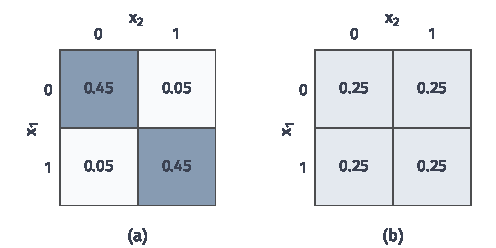
\includegraphics[width=84mm]{figures/07-probability/07-distribution-optimization/matplotlib/dapx-table-product/figure.pdf}
 \caption{结构限制删去依赖。(a)式~\eqref{eq:dapx-table}的目标概率表，行是$x_1$，列是$x_2$，颜色越深概率越大。(b)它的两个边缘都是$(\tfrac12,\tfrac12)$，边缘乘积在四格上都是$0.25$。}
 \label{fig:dapx-table-product}
\end{BookInlineFigure}

这里丢掉的东西可以用第~\ref{chap:information-measures}章的互信息度量。目标与它的边缘乘积之间的KL散度就是$I(X_1;X_2)$，计算得
\[
 D_{\mathrm{KL}}(\Pi\Vert\Pi_1\otimes\Pi_2)=0.9\ln\frac{0.45}{0.25}+0.1\ln\frac{0.05}{0.25}=0.9\ln1.8-0.1\ln5\approx0.3681 .
\]
第~\ref{sec:dapx-mean-field}节将证明，在按目标加权的方向上，这个数恰好是乘积候选所能达到的最小KL；在另一个方向上，最优的乘积分布并不是边缘乘积。

\paragraph{支持、参数范围与可积性}
选定候选集合后，还要检查逼近目标在这两个集合之间是否有意义。第一项检查是支持。设目标是$\operatorname{Exp}(1)$，密度在$x<0$处为零，候选集合是全体一维高斯分布。每个高斯分布都给$(-\infty,0)$正概率，所以$Q\ll\Pi$不成立；按第~\ref{chap:distribution-comparison}章的约定，$D_{\mathrm{KL}}(Q\Vert\Pi)=+\infty$对每个候选成立，这个方向的KL无法区分任何两个候选。另一个方向$D_{\mathrm{KL}}(\Pi\Vert Q)$则对每个高斯候选有限，因为高斯密度处处为正。图~\ref{fig:dapx-support}(a)中红色区域就是候选有质量而目标没有的部分。

第二项检查是参数范围。参数必须落在使候选成为合法分布的集合内：标准差为正，概率表的分量非负且和为$1$，协方差矩阵对称正定，混合权重在单纯形上。优化时这些都是约束，第~\ref{sec:dapx-gradient}节会用重新参数化来自动满足它们。

第三项检查是可积性。绝对连续只保证对数比几乎处处有限，不保证它的期望有限。取目标为标准Cauchy分布，候选为$\mathcal{N}(0,1)$。两个密度处处为正，但
\[
 \ln\frac{\pi(x)}{q(x)}=\frac{x^{2}}{2}-\ln(1+x^{2})+\ln\sqrt{\frac{2}{\pi}} ,
\]
它在Cauchy分布下的期望含有$\mathbb{E}_{\Pi}[X^{2}]=+\infty$，所以$D_{\mathrm{KL}}(\Pi\Vert Q)=+\infty$。把$\mathcal{N}(0,1)$换成任何其他高斯分布，对数比中仍有$x^{2}$的正系数项，结论不变：这个方向对全体高斯候选都是无穷大。反方向的被积函数在高斯权重下迅速衰减，$D_{\mathrm{KL}}(Q\Vert\Pi)$有限，数值积分给出约$0.259$。

\begin{BookInlineFigure}
 \centering
 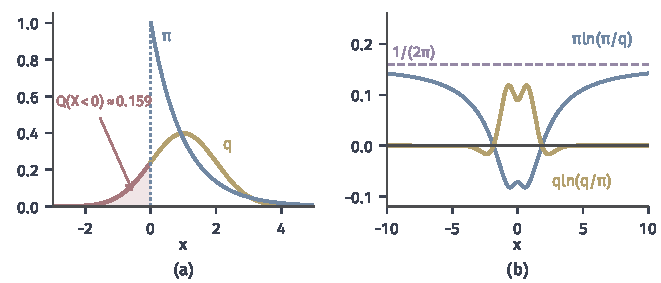
\includegraphics[width=112mm]{figures/07-probability/07-distribution-optimization/matplotlib/dapx-support/figure.pdf}
 \caption{逼近目标可能对所有候选都无穷大。(a)目标$\operatorname{Exp}(1)$（蓝）与候选$\mathcal{N}(1,1)$（黄），红色区域是候选落在$x<0$的质量$\Phi(-1)\approx0.159$，目标在那里没有质量，所以$D_{\mathrm{KL}}(Q\Vert\Pi)=+\infty$。(b)目标为标准Cauchy分布、候选为$\mathcal{N}(0,1)$时两个方向的被积函数：蓝线$\pi\ln(\pi/q)$在远处趋于常数$1/(2\pi)$（紫色虚线），积分发散；黄线$q\ln(q/\pi)$迅速衰减。}
 \label{fig:dapx-support}
\end{BookInlineFigure}

图~\ref{fig:dapx-support}(b)显示了无穷大的来源：Cauchy分布在远处的密度约为$1/(\pi x^{2})$，乘上对数比中的$x^{2}/2$后趋于常数$1/(2\pi)$，在整条直线上积分必然发散。这两个例子说明，KL目标是否有限取决于目标、候选与方向三者的组合。确定候选集合时就要检查它，不能留到优化出问题时再发现。
